\documentclass[border=8pt]{standalone}
\usepackage{fontspec}
\setmainfont{Source Serif 4}
\usepackage{pgfplots}
\pgfplotsset{compat=1.18}
\definecolor{qbase}{RGB}{31,86,160}

\begin{document}
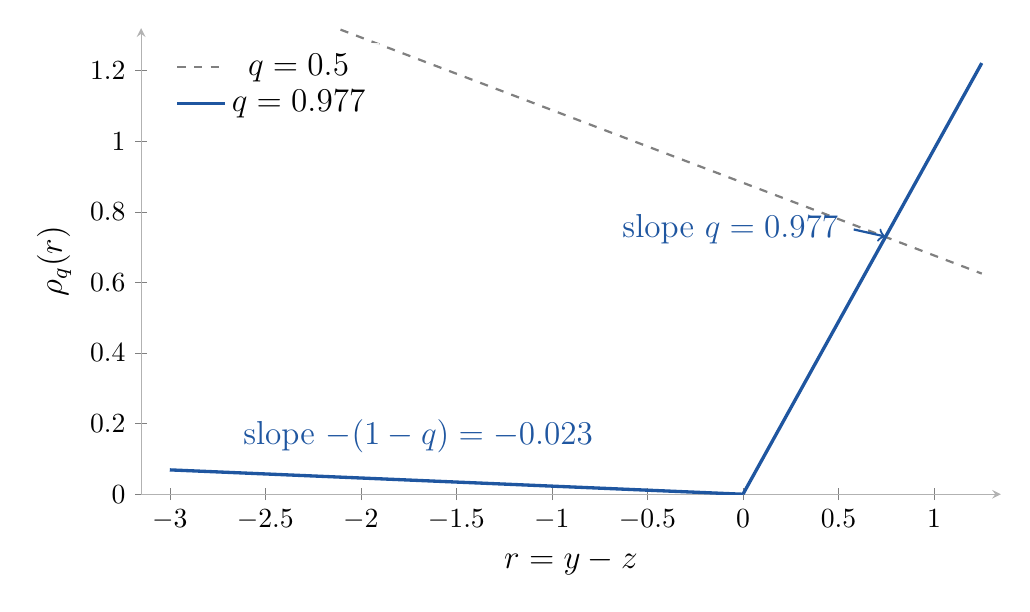
\begin{tikzpicture}
\begin{axis}[
  width=12.5cm, height=7.5cm,
  axis lines=left,
  xlabel={$r = y - z$}, ylabel={$\rho_q(r)$},
  xmin=-3.15, xmax=1.35, ymin=0, ymax=1.32,
  label style={font=\large},
  tick label style={font=\normalsize},
  legend style={at={(0.03,0.97)}, anchor=north west, font=\large, draw=none,
                fill=white, fill opacity=0.9, text opacity=1},
  axis line style={gray!60},
]
\addplot[domain=-3:1.25, samples=2, dashed, thick, gray]
  {0.5*abs(x)};
\addlegendentry{$q = 0.5$}
\addplot[domain=-3:0, samples=2, very thick, qbase] {0.023*(-x)};
\addlegendentry{$q = 0.977$}
\addplot[domain=0:1.25, samples=2, very thick, qbase, forget plot] {0.977*x};
% slope annotations
\node[qbase, font=\large, anchor=east] at (axis cs:0.55,0.75) {slope~$q = 0.977$};
\draw[->, qbase, thick] (axis cs:0.58,0.75) -- (axis cs:0.745,0.73);
\node[qbase, font=\large, anchor=south] at (axis cs:-1.7,0.09) {slope~$-(1-q) = -0.023$};
\end{axis}
\end{tikzpicture}
\end{document}
